\section{Runtime Performance}
\label{sec:eval-performance}

The second research question concerns the sensing pipeline: whether a real Tobii stream is converted into oculomotor events within a latency budget that preserves live adaptation, in a manner that is inspectable and reproducible.
We report the sensing throughput and validity first, then the transport latency against the budget fixed in \cref{sec:non-functional-requirements}.

Across the eight sessions the eye tracker delivered a steady stream at its rated rate.
The achieved sampling rate, computed from the device timestamps, lay between \SI{89.4}{\hertz} and \SI{90.1}{\hertz}, and the gaze-validity rate ranged from 92.5\% to 98.0\%.
\Cref{fig:eval-sensing} shows the achieved rate and validity per session, and \cref{fig:eval-intersample} shows the inter-sample interval, which clusters tightly at the nominal period of \SI{11.1}{\milli\second}.
The calibration that gated each session, the sub-flow shown in \cref{fig:impl-calibration}, passed with an average accuracy between \ang{0.30} and \ang{0.69} and an average precision between \ang{0.08} and \ang{0.33}.

\begin{figure}[htbp]
\centering
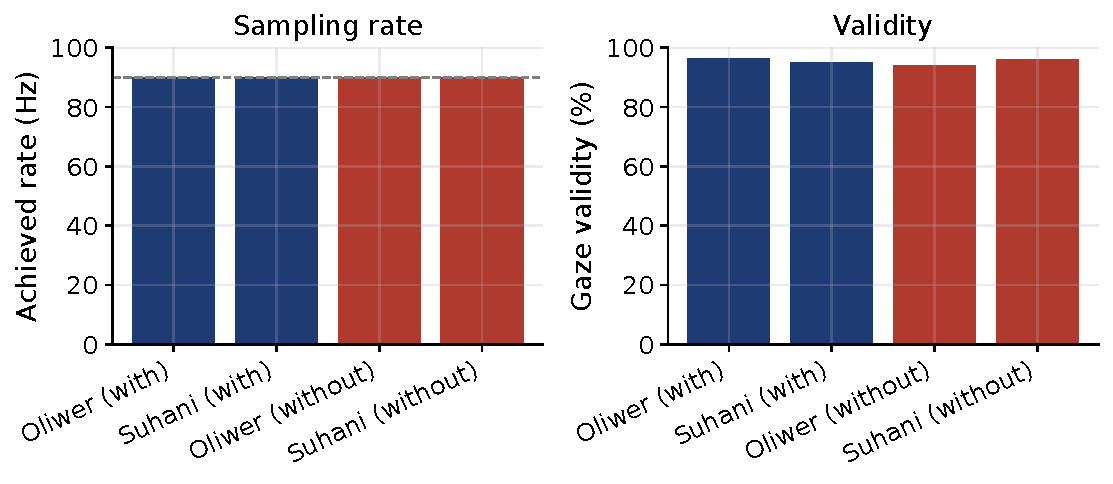
\includegraphics[width=0.92\linewidth]{Chapters/07_Evaluation/eval-sensing-rate-validity.pdf}
\caption{Achieved sampling rate and gaze validity for each of the eight sessions. The achieved rate sits at the tracker's nominal \SI{90}{\hertz} and validity stays above 92\% throughout.}
\label{fig:eval-sensing}
\end{figure}

\begin{figure}[htbp]
\centering
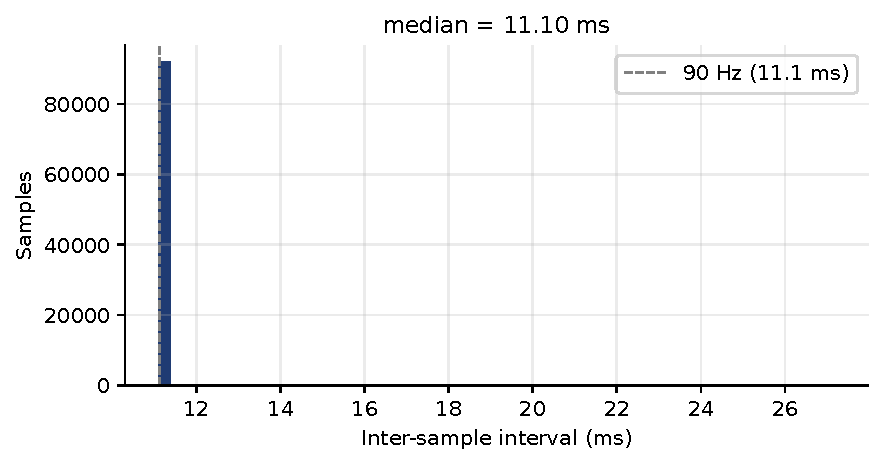
\includegraphics[width=0.78\linewidth]{Chapters/07_Evaluation/eval-inter-sample-interval.pdf}
\caption{Distribution of the interval between consecutive gaze samples, pooled across sessions and measured from the device clock. The mass concentrates at the nominal \SI{11.1}{\milli\second} period of a \SI{90}{\hertz} stream.}
\label{fig:eval-intersample}
\end{figure}

The low-latency requirement (NFR2) fixes a budget of \SI{100}{\milli\second}, the threshold at which an interface response ceases to be perceived as instantaneous \cite{miller1968response, nielsen1993responsetime} and well within the duration of a single reading fixation \cite{rayner1998eyemovements}.
The telemetry record carries the round-trip time between each client and the backend.
For the participant client the median round trip was \SI{1}{\milli\second} and the 95th percentile \SI{3}{\milli\second}, and for the researcher client the median was \SI{1}{\milli\second} and the 95th percentile \SI{8}{\milli\second}.
No sample in either stream exceeded the \SI{100}{\milli\second} budget.
\Cref{fig:eval-rtt} shows the two distributions against the budget.

\begin{figure}[htbp]
\centering
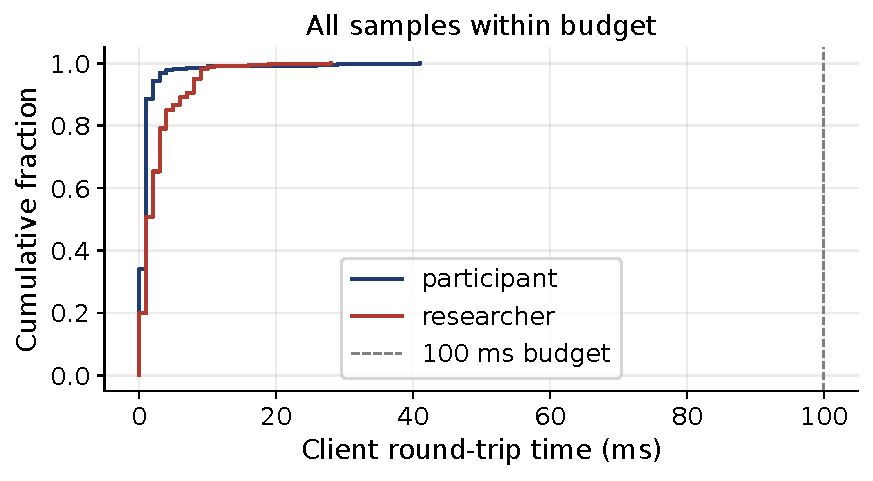
\includegraphics[width=0.78\linewidth]{Chapters/07_Evaluation/eval-client-rtt.pdf}
\caption{Cumulative distribution of client round-trip time for the participant and researcher clients, against the \SI{100}{\milli\second} budget. Every sample falls within budget.}
\label{fig:eval-rtt}
\end{figure}

The round trip reported above is the transport latency between a client and the backend over the local loopback of the single-machine deployment (\cref{sec:eval-setup}).
The platform also records the in-process decision-pipeline latency, from the freshest gaze sample to the dispatch of an automated decision, and the out-of-process round-trip latency to an external decision provider, each on a single backend clock.
Both are recorded only when an automated decision strategy is active.
The eight sessions were operated in manual mode, in which the researcher applies interventions directly, so neither latency was exercised and the telemetry contains no decision-latency samples.
The instrumentation is therefore present and available but unexercised in this dataset, and we treat the question it would answer as future work in \cref{ch:discussion}.
